\documentclass[main.tex]{subfiles}
\begin{document}

\section*{8 October 2019}

\subsubsection{An ansatz for the LAWE}

Last lecture we started talking about linearization \& perturbation theory.

We use a complex spinning ansatz, which is by itself not physical, however its conjugate is also a solution so after we have found a solution we just need to take the real part.

Substituting \(\zeta (m, t) = \eta (m) \exp(i \sigma t)\) into the LAWE we find that the exponentials simplify: 
%
\begin{align}
-r \sigma^2 \eta  =
4 \pi r^2 \eta \pdv{}{m} \qty((3 \Gamma_1 - 4)P)+
\frac{1}{r} \pdv{}{m} \qty(16 \pi^2 \Gamma_1 P \rho r^6 \pdv{\eta }{m} )  
\,.
\end{align}

Since we have an explicit \(r\), it is convenient to rewrite this in the Eulerial formalism, using the continuity equation: we get 
%
\begin{subequations}
\begin{align}
- r \sigma^2 \eta &= 
\frac{\eta }{\rho } \pdv{}{r} \qty((3\Gamma_1 - 4) P)
+ \frac{1}{r^3 \rho } \pdv{}{r} \qty(\Gamma_1 P r^{4} \pdv{\eta }{r})  \\
\sigma^2 \eta  &= - \hlc{green}{\frac{\eta }{\rho r} \pdv{}{r} \qty(3 \Gamma_1 P - 4P )} -\hlc{cyan}{\frac{1}{r^{4} \rho } \pdv{}{r} \qty(\Gamma_1 P r^{4} \pdv{\eta }{r})}
\,, \label{eq:linear-operator-LAWE}
\end{align}
\end{subequations}
%
\todo[inline]{Slide 4.37: there is a minus sign missing, right?}

We will have analytic solutions for the adiabatic case, with the additional hypotheses of either \(\Gamma_1 = 4/3\) or \(\Gamma_1 > 4/3\) and homogeneity.

[The justification of the adiabatic approx might be asked at the exam.]

\subsubsection{Boundary conditions for the LAWE}

What are the boundary conditions we should set? The final result is:
%
\begin{enumerate}
    \item \(\delta r = 0\) at \(r = 0\);
    \item \(\pdv*{\eta}{r} = 0 \) at \(r=0\);
    \item \((4 + R^3 \sigma^2 / (GM)) \eta + \delta P / P = 0\) at \(r =R\);
    \item \(\eta = \delta r / r = 1\) at \(r = R\).
\end{enumerate}

Let us show why. The first condition has an immediate physical basis: there cannot be radial displacement at \(r=0\) since there is nowhere to go at \(r<0\), and if there was positive radial displacement \(\delta r\) it would mean there is a vacuum in the region \(r<\delta r \), which is unphysical because of the pressure there.

So, by the first condition, we need the term 
%
\begin{align}
\hlc{cyan}{\frac{1}{r^4 \rho } \pdv{}{r} \qty(\Gamma_1 P r^{4} \pdv{\eta }{r})}
= \frac{\Gamma_1 P}{\rho } \pdv[2]{\eta }{r}
+ 4 \frac{\Gamma_1 P}{\rho r} \pdv{\eta}{r} 
+ \frac{\Gamma_1 }{\rho } \pdv{\eta }{r} \pdv{P}{r}
+ \frac{P}{\rho } \pdv{\eta }{r} \pdv{\Gamma_1}{r}
\,
\end{align}
%
to be well behaved (nonsingular) at \(r=0\). 

We know that \(\pdv*{P}{r}\) and \(\pdv*{\Gamma_1}{r}\) are zero at \(r=0\), so we can neglect the terms containing them. This is because any physical quantity must approach \(r=0\) with zero \(\dv*{}{r}\) slope, in order for it to be differentiable at the center.

% Let us show this: we write the momentum conservation equation in the Eulerian form, 
% %
% \begin{align}
% \pdv{P}{r} = - \frac{Gm \rho }{r^2}
% \,,
% \end{align}
% %
% and look at the asymptotic behaviour at \(r \rightarrow 0\): \(\rho \) and \(G\) are finite, while \(m\) and \(r^2\) go to zero. We know that \(m  \sim r^3\), therefore globally the behaviour is \(r^3/r^2 = r \rightarrow 0\).

% Also, we know that \(P = \rho^{\Gamma_1 }\). So, let us write \(\pdv*{P}{r}\): 
% %
% \begin{align}
% \pdv{}{r} \exp(\Gamma_1 \log \rho )
% = \exp(\Gamma_1 \log \rho) \qty(\log \rho \pdv{\Gamma_1  }{r} + \Gamma_1 \pdv{}{r} \log \rho ) = 0
% \,,
% \end{align}
% %
% \todo[inline]{prove that \(\pdv*{\Gamma_1}{r} =0\) for \(r=0\)}

In the second term we have a division by \(r\): in order for it not to diverge we must ask that \(\pdv*{\eta }{r} =0\) at \(r=0\). 

Since \(\eta \) is \(\zeta \) times a phase, this also means that \(\pdv*{\zeta }{r} =0 \) at \(r=0\). 
We can plug this into the linearized continuity equation, the Eulerian form of \eqref{eq:linearized-continuity}: 
%
\begin{align}
\frac{ \delta \rho }{\rho } &= - 3\zeta - r\pdv{\zeta }{r} \\
0=\pdv{\zeta }{r} &= - \frac{1}{r} \qty(3\zeta + \frac{ \delta \rho }{\rho })  \\
\implies 0 &= 3\zeta + \frac{ \delta \rho }{\rho }
\,,
\end{align}
%
into which we can substitute the linearized adiabatic expressions for the temperature and pressure perturbations \eqref{eq:linearized-adiabatic-energy-conservation}: so we find 
%
\begin{align}
3\zeta = - \frac{1}{\Gamma_1 } \frac{ \delta P }{P}
= - \frac{1}{\Gamma_3 -1} \frac{ \delta T}{T}
\,,
\end{align}
%


We use the Eulerian form of the momentum conservation \eqref{eq:linearized-momentum-conservation} to figure out the surface boundary conditions: it reads 
%
\begin{align}
r \sigma^2 \eta &= 
\frac{1}{\rho } \qty(P \pdv{}{r} \qty(\frac{ \delta P}{P}) 
+ \frac{ \delta P }{P } \pdv{P}{r} 
+ 4 \eta  \pdv{P}{r})  \\
\pdv{}{r} \qty(\frac{ \delta P}{P}) &= \frac{\rho}{P} 
\qty(r \sigma^2 \eta ) - \frac{1}{P} \qty(\frac{ \delta P}{P} \pdv{P}{r} + 4 \eta  \pdv{P}{r})  \\
&= \frac{\rho r \sigma^2 \eta }{P}
- \frac{ \delta P}{P} \pdv{\log P}{r}
- 4 \eta \pdv{\log P}{r}  \\
&= -\pdv{\log P}{r} \qty(- \frac{\rho r \sigma^2 \eta }{\pdv*{P}{r}}
+ 4 \eta
+ \frac{ \delta P}{P} 
) 
\,,
\end{align}
%
since we assumed that all perturbations are \emph{in phase} to the radial one, and thus wrote them all as proportional to \(\exp(i \sigma t)\), which then simplified.
We define the \emph{pressure scale height} as:

\begin{equation}
  H_P = - \qty(\pdv{\log P }{r} )^{-1}\,,
\end{equation}
%
it represents ``how far we should move in the star for the pressure to change \(e\)-fold''.

We insert this into the equation; also we use the Eulerian momentum conservation equation 
%
\begin{align}
\pdv{P}{r} = -\rho \frac{Gm}{r^2}
\,,
\end{align}
%
so that we find 
%
\begin{align}
\pdv{}{r} \qty(\frac{ \delta P}{P}) =
\frac{1}{H_P} \qty(
\qty(
4 + \frac{r^3 \sigma^2}{ Gm}
) \eta 
+ \frac{ \delta P }{P }
)
\,,
\end{align}
%

Since outside the star the pressure is zero, we must have that \(H_P \rightarrow 0\) when \(r \rightarrow R\): the pressure must change by an infinite number of \(e\)-folds to reach zero, so the displacement needed for a single \(e\)-fold change must go to zero. Therefore, the term multiplying \(1/H_P\) must also go to zero to avoid divergences: so we ask 
%
\begin{align}
\qty(4 + \frac{r^3 \sigma^2 }{Gm}) \eta + \frac{ \delta P}{P} \rightarrow 0 
\,
\end{align}
%
as \(r \rightarrow R\). Since we are considering the mass variable at the edge of the star, we also must have \(m=M\).

The last condition, \(\eta = \delta r / r = 1\) at \(r=R\) comes from the fact that we want our study to give us \emph{periods}, not \emph{amplitudes}: we cannot find those out, so we normalize in a way that is convenient. The LAWE is 1-homogeneous!

\subsubsection{Solving the LAWE}

The LAWE can be written compactly with a linear operator \(\mathcal L\):

\begin{equation}
  \mathcal L (\eta) = \sigma^2 \eta\,,
\end{equation}
%
where the expression for \(\mathcal{L}\) can be read off equation \eqref{eq:linear-operator-LAWE}. The equation is in the form of a Sturm-Liouville differential equation; in general those have the form 
%
\begin{align}
\pdv{}{r} \qty(p(r) \pdv{\eta }{r}) + \lambda t(r) \eta 
- s(r) \eta  = 0 
\,.
\end{align}

\todo[inline]{Figure out signs! Why does nothing make sense?}

So, the eigenvalue \(\sigma^2\) is the square of the pulsation.
There are infinitely many solutions to the LAWE, only some (finitely many?) fulfill the boundary condition.
The eigenvalues are real since \(\mathcal L\) is Hermitian,  and they have a wavefunction associated: \(\eta_m (r)\) corresponding to \(\sigma_m ^2\).

If \(\sigma^2 > 0\) we have an oscillating solution, if \(\sigma^2 <0 \) we have an exponential collapse or explosion since the solution is proportional to \(\exp(i \sigma t)\).

We label solutions by \emph{radial order} \(m \in \mathbb{N}\): \(m=0\) has the lowest frequency, and then we have overtones.
We choose the labels so that \(\sigma_{m_1} < \sigma_{m_2} \iff m_1 < m_2\).

The radial order \(m\) is also the number of nodes.

The eigenfunctions are orthogonal wrt the scalar product

\begin{equation}
  \braket{\eta_m}{\eta_n} = \int _{0}   ^{R} \eta_m \eta_n \rho r^4 \dd{r} = f(n) \delta_{nm}
\end{equation}

\todo[inline]{Possibly there is a \(4 \pi\) missing in order for this to be consistent with the following?}

The functions \(\zeta_m\) are orthogonal wrt the same product. The system is linear: we can write a general solution as a superposition.

We can define the moment of inertia:

\begin{equation}
  J_m = \int _{0}   ^{M} \abs{\zeta_m}^2 r^2 \dd{m}
\end{equation}

and then we can recover the eigenvalue by:

\begin{equation}
  \sigma_m^2 = \frac{1}{J_m} \int_0^M \zeta_m ^* \mathcal L \zeta_m r^2 \dd{m}
  = \frac{\ev{\mathcal{L}}{\zeta_{m}}}{\braket{\zeta_{m}}{\zeta_{m}}}
\end{equation}

\subsection{Simplifications}

\subsubsection{Period-mean density relation}

If \(\eta = \const\), and \(\rho \) and \(\Gamma_1\) are also constanst, we can remove the \(\pdv*{\eta }{r}\) terms: so we have 
%
\begin{align}
\sigma^2 \eta + \frac{\eta }{\rho r} \pdv{}{r} \qty(P \qty(3 \Gamma_1 - 4)) &= 0  \\
\sigma^2 &= - \frac{3 \Gamma_1 - 4}{\rho r} \pdv{P}{r}  \\
\sigma^2 &= \qty( 3\Gamma_1 -4 ) \frac{Gm}{r^3}
\,,
\end{align}
%
and by inserting the mean density formula \(\overline{\rho} = M / \qty(4 \pi R^3 / 3)\) we get the period-mean density relation: \(\sigma = 2 \pi / T\), so we have \(T^{-2} \propto \overline{\rho}\), the period-mean density relation. 

Actually, this simplified model gives us \(m / r^3 = \const\): the density in this case must be constant and equal to \(\overline{\rho}\) (even if we did not use the assumption before). 
The precise relation is given by 
%
\begin{align}
T^2 \overline{\rho} = \frac{3 \pi }{\qty(3 \Gamma_1 -4) G}
\,,
\end{align}
%


\subsubsection{Polytropic model}

It is a gas sphere with the following constitutive equaition:

\begin{equation}
  P = K_n \rho^{1 + 1/n} = K_n \rho^{\frac{n+1}{n}}
\end{equation}
%
with varying \emph{polytropic} index \(n\).

\begin{bluebox}
This can be derived as a solution for the Lane-Emden equation, which comes from Poisson's equation for the gravitational potential: so we do the following manipulation 
%
\begin{align}
\nabla^2 \Phi  &= 4 \pi G \rho  \\
\frac{1}{r^2} \dv{}{r} \qty(r^2 \dv{\Phi }{r}) &= 4 \pi G \rho  \marginnote{Laplacian in spherical coordinates under spherical symmetry}[-1cm]\\
-\frac{1}{r^2}\qty(\frac{r^2}{\rho } \dv{P}{r}) &= 4 \pi G \rho   \marginnote{Used the hydrostatic equilibrium equation}\\
\dv{}{r} \qty(\frac{r^2}{\rho } \dv{P}{r}) &= - 4 \pi G \rho r^2
\,,
\end{align}
%
so if we assume \(\rho = \rho_{c} \theta^{n}\) the polytropic equation of state will read 
%
\begin{align}
P = K_n \rho^{1 + 1/n} = K_n \rho_{c}^{1 + 1/n} \theta^{n (1 + 1/n)}
= K_n \rho_{c}^{1 + 1/n} \theta^{n+1}
\,,
\end{align}
%
where \(\rho_{c}\) is the central density, so we have \(\theta (r=0) = 1\) and \(\theta' (r=0) =0\). Inserting this into Poisson's equation gives us 
%
\begin{align}
\dv{}{r} \qty(\frac{r^2}{\rho_{c} \theta^{n}}
\dv{}{r} \qty(K_{n} \rho_{c}^{1 + 1/n} \theta^{n+1})) &=-4 \pi G \rho r^2  \\
\dv{}{r} \qty(r^2 (n+1) K_n \rho_{c}^{1/n} \dv{\theta }{r}) & = - 4 \pi G \rho r^2
\,,
\end{align}
%
so we can adimensionalize the radial coordinate by putting inside of it all the numbers: \(r = \alpha \xi \), with \(\alpha \) chosen so that the equation turns into
%
\begin{align}
\frac{1}{\xi^2} \dv{}{\xi } \qty(\xi^2 \dv{\theta }{\xi })
+ \theta^{n} = 0
\,.
\end{align}

This is always solvable, and it is solvable analytically for certain values of \(n\). 

\end{bluebox}

It models spheres with different mass distributions:
\(n=0\) is constant density, \(n=5\) is infinite central density, \(n=3\) is the Eddington standard model, which is reasonable for the Sun and stars on the main sequence.

With these assumptions we can explicitly solve for the wavefunctions, and make predictions of the fractional modulus of the oscillations at a certain radius wrt the modulus at the surface (which can be found only experimentally).

The overtones die out toward the center even faster than the fundamental: these oscillations are very much a \emph{surface phenomenon}.

Beyond the \(\eta\)s we can also plot the pressure perturbations: these will not be normalized.

\begin{bluebox}
Slide 4.108: What is \(\omega \)? Should we not have \(\sigma = \omega \) of the mode? It seems like \(\mathcal{P}\) is the period, and the numbers are consistent with \(\mathcal{P} = 2 \pi / \sigma \)

Answer, from the first equation in Schwarzschild 1941\footnote{\url{https://ui.adsabs.harvard.edu/abs/1941ApJ....94..245S/abstract}}: \(\omega \) and \(\sigma \) are related by 
%
\begin{align}
  \omega = \frac{\sigma}{\sqrt{\pi G \Gamma_1 \rho_{0c}}}
  \,,
\end{align}
%
so \(\omega \) is adimensional: it is, in a certain sense, an adimensionalized frequency. From the data in slide 4.108 we can derive the value of \(\Gamma_1 \rho_{0c} = (\sigma / \omega )^2 / (\pi G) \approx \SI{5.184e14}{kg/m^3}\).
\end{bluebox}

\subsubsection{Numerical RR Lyrae models}

We integrate the stellar structure equations numerically, so instead of a simple polytropic equilibrium model our equilibrium model is numerical. 
This is done looking at an RR Lyrae variable stars.
\todo[inline]{What are their characteristics?}

\begin{figure}[ht]
\centering
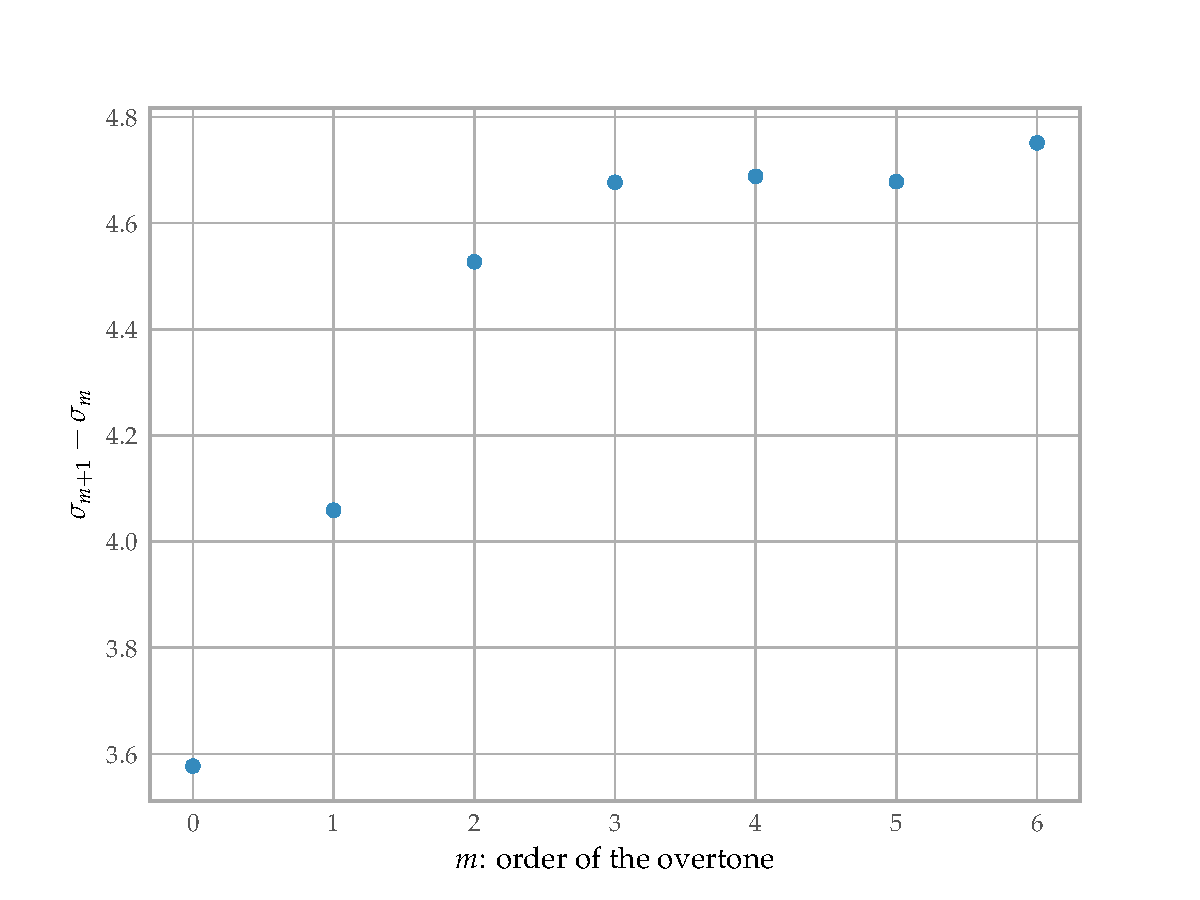
\includegraphics[width=\textwidth]{RR_Lyr_frequency_differences.pdf}
\caption{RR Lyrae frequency differences. The frequencies are measured in \SI{}{rad / d}.}
\label{fig:RR_Lyr_frequency_differences}
\end{figure}

We find that the ratio between the period of the fundamental and of the first overtone is around \(P_1 / P_0 \approx \num{.743} \divisionsymbol \num{.745}\) in observed RR Lyrae, while the LAWE model predicts \(\num{.731}\). 
The observed period is around \(P_0 \approx \SI{.5668}{d}\), while the model predicts \(P_0 \sim \SI{.6454}{d}\). 

We can see that \(\sigma_m - \sigma_{m-1} \approx \const\) when \(m\) gets large, see figure \ref{fig:RR_Lyr_frequency_differences}.
  

The wavefunctions die out faster than the polytropic model when \(r \rightarrow 0\).

There are ``bumps'' in the pressure perturbation plot: these are the partial ionization regions of \ce{H} and \ce{He}.

These appear because we start from a solution of the stellar structure equations, where all the properties of stellar matter were used, to start off with the LAWE.

\section{Non-adiabatic oscillations}

\subsection{Driving and damping layers}

How can we tell, theoretically, how stable and how wide the various modes are?
We expect to see the stable modes, and not to see the unstable ones.

Let us start from the Lagrangian momentum conservation:

\begin{equation}
    \pdv[2]{r}{t} = - 4 \pi r^2 \pdv{P}{m} - \frac{Gm}{r^2}
\end{equation}

and apply to it the identity: \(\frac[i]{1}{2} \pdv{}{t} v^2 = \pdv{r}{t} \pdv[2]{r}{t}\), by multiplying everything by \(\pdv*{r}{t} \), and then we integrate everything with respect to \(m\): we find 
%
\begin{align}
\int_{M} \frac{1}{2} \pdv{}{t} \qty(v^2) \dd{m} = 
\hlc{olive}{- \int_{M} 4 \pi r^2 \pdv{P}{m} \dd{m} }
\hlc{teal}{- \int_{M} \frac{Gm}{r^2} \dd{m}}
\,,
\end{align}
%


Now we apply some manipulations: first of all, the following: 
%
\begin{align}
\hlc{teal}{\int_{M} \qty(- \frac{Gm}{r^2} \pdv{r}{t}) \dd{m}} &= 
\int_{M} \pdv{}{t} \qty(\frac{Gm}{r}) \dd{m}  \\
&= \dv{}{t} \int_{M} \frac{Gm}{r} \dd{m}  \\
&= \hlc{teal}{- \dv{\Omega }{t}}
\,
\end{align}
%
where \(\Omega \) is the total gravitational potential energy, while 
%
\begin{align}
\hlc{olive}{- \int_{M} 4 \pi r^2 \pdv{P}{m} \pdv{r}{t} \dd{m}} &= 
- \int_{M} \pdv{}{m} \qty(4 \pi r^2 P \pdv{r}{t}) \dd{m}
+ \int_{M} P \pdv{}{m} \qty(4 \pi r^2 \pdv{r}{t}) \dd{m}  \\
&= - \underbrace{\eval{4 \pi r^2 P \pdv{r}{t}}_{m=0}^{m=M}}_{=0}
+ \int_{M} \frac{4 \pi }{3} P \pdv{}{m} \pdv{}{t} \qty(r^3) \dd{m}  \\
&= \int_{M} P \pdv{}{t} \underbrace{\qty(4 \pi r^2 \pdv{r}{m})}_{1 / \rho } \dd{m}  \marginnote{Commuted \(m\) and \(r\) derivatives}\\
&= \hlc{olive}{\int_{M} P \pdv{}{t} \qty(\rho^{-1}) \dd{m}}
\,,
\end{align}
%
so in the end we get 
%
\begin{equation}
\pdv{}{t} \int_M \frac{v^2}{2} \dd{m} =
\hlc{teal}{- \dv{\Omega}{t} } +
\hlc{olive}{\int_M P \pdv{}{t} \frac{1}{\rho} \dd{m}}
\end{equation}

We integrate in time over a pulsation period, which cancels out the gravitational potential term which is conservative: 
%
\begin{align}
-\int_{\Pi } \dv{\Omega }{t} \dd{t} = 0
\,.
\end{align}

If we also divide by the period, we are computing an average over a period \(\Pi \). The term 
%
\begin{align}
\expval{\pdv{}{t} \int_{M} \frac{v^2}{2} \dd{m}}_{\Pi }
= \frac{1}{\Pi } \int_{\Pi } \pdv{}{t} \int_{M} \frac{v^2}{2} \dd{m} \dd{t} = \frac{ \Delta E _{\text{kin}}}{\Pi }
\,
\end{align}
%
is the average power converted to kinetic energy; the variation in kinetic energy is also the work done on the system: \(\Delta E _{\text{kin}} = W\). So, taking the average on both sides of the equation we get
%
\begin{equation} \label{eq:driving-damping-layers-1}
\expval{\dv{W}{t}}_\Pi = \frac{1}{\Pi} \int_\Pi \int_M   P \pdv{}{t} \qty(\frac{1}{\rho}) \dd{m} \dd{t}.
\end{equation}

Some layers will provide energy to the oscillation motion (\emph{drive} it), some others will \emph{damp} it.
These are characterized by the sign of their contribution the RHS of this equation.

If it is positive, we have instability since more and more work is being done one the star every period; if it is negative the pulsations will tend to die out, giving stability, since they lose kinetic energy every pulse.

The average time scale of change of the perturbations is

\begin{equation}
  \kappa \defeq \frac{1}{\tau} = -\frac{1}{2} \frac{\expval{\dv*{W}{t}}_\Pi}{\expval{ \delta \psi}_\Pi }
\,,
\end{equation}
%
where \(\expval{ \delta \psi }\) is the ``average pulsational energy per pulsation cycle'': 
\todo[inline]{
so, the integral of the absolute value of \(\dv*{W}{t}\)?
This \(\psi \) was not defined... 

Also, this way \(\tau \) can be negative: maybe the proper definition is \(\tau = 1/ \abs{\kappa }\)?
}

So, if \(\kappa < 0\) we are looking at a driving layer, since then \(\expval{ \dv*{W}{t}} >0\), while \(\kappa > 0\) means we are in a damping layer. 

The term \(\expval{\dv*{W}{t}}_\Pi \) can also be interpreted as the net heat gain fed into mechanical work during a pulsation cycle: this can be derived from the first law of thermodynamics (written in its per-unit-mass form, and with the differentials being applied to time derivatives): 
%
\begin{align}
\dv{Q}{t} = \dv{E}{t} + P \dv{(\rho^{-1})}{t}
\,,
\end{align}
%
so if this is averaged over a period the internal energy change is approximately zero (thermal (i.\ e.\ internal) energy changes on the thermal timescale, which is much longer than the dynamical timescale), so we have 
%
\begin{align}
\expval{\dv{Q}{t}}_{\Pi } = \expval{P \dv{}{t} (\rho^{-1})}
\,,
\end{align}
%
and therefore we can rewrite equation \eqref{eq:driving-damping-layers-1} as 
%
\begin{align}
\expval{\dv{W}{t}}_{\Pi } = \frac{1}{\Pi } \int_{\Pi } \int_{M} \dv{Q}{t} \dd{m} \dd{t}
\,,
\end{align}
%
where \(Q\) is a heat per unit mass, so its integral in \(\dd{m}\) is the total heat change across all stellar layers.

In the adiabatic case, we had 
%
\begin{align}
\pdv{}{t}\qty( \frac{\delta P}{P} - \Gamma_1 \frac{\delta \rho}{\rho}) =0
\,,
\end{align}
%
(see equation \eqref{eq:perturbed-linearized-energy-log-pressure}, in which we neglected the heat variation terms in the adiabatic case) so the perturbations were in phase.

Now we add a term to the time derivatives: the pressure and density perturbations will stop being in phase. The sign of the heat variation term gives us the difference between \emph{driving} heat transfer and \emph{damping} heat transfer. Equation \eqref{eq:perturbed-linearized-energy-log-pressure} will now look like 
%
\begin{align}
\pdv{}{t} \frac{ \delta P}{P} = \Gamma_1 \frac{ \delta \rho }{\rho } + \frac{P}{\rho } (\Gamma_3 -1) \delta \dv{Q}{t}
\,,
\end{align}
%
so the insants of minimum pressure and minimum density will not be synchronized anymore, since there is that extra \(\dv*{Q}{t}\) term. 

In a PV diagram, we can see that these correspond to right and left oriented loops (as opposed to the loops with zero total signed area we had in the adiabatic case).

The total work performed on the star is given by the area of the loops: the area is positive for a loop going clockwise, and negative for a loop going counter-clockwise.

If the term \(\delta \qty(\dv*{Q}{t})>0\) we are looking at a \emph{driving layer}, since at the time of maximum compression (\(\pdv*{}{t} (\delta \rho  / \rho ) = 0\)) we will have \(\pdv*{}{t} \qty(\delta P / P) > 0\): the maximum pressure perturbation will happen as the layer is expanding, so the expansion will be amplified.
The symmetric reasoning gives us the fact that if \(\delta \qty(\dv*{Q}{t}) < 0\) we have a \emph{damping layer}. 

There tend to be more driving layers in the outer parts of the star, especially peaking in power generation in the partial Helium and Hydrogen ionization regions.  

\todo[inline]{What is going on in these regions? Why do they act this way?}

\begin{bluebox}
The star is effectively a themal engine converting heat into work; this will result in an increased overall entropy of the star, and a smoothing of its temperature gradient, however:
%
\begin{enumerate}
\item the time scales on which this process occurs are much larger than the time scales on which oscillating motions are created and destroyed (specifically, the entropy changes on the thermal time scale);
\item then energies of the oscillations are much smaller than the global thermal energy of the star.
\end{enumerate}
%
therefore this process is typically not relevant.
\end{bluebox}

\end{document}
